\section{Add And Remove Applications}
\label{sec:add_and_remove_applications}
This section will solve the following user story which was estimated as \pmedhigh~by the PO:

\userstory{As a guardian, I would like the launcher to tell me how to add applications if none are active, such that it is easier for a new guardian.}
In the GIRAF launcher, a guardian must specify which apps should be visible from the home screen.
This is the case for both himself and any citizens in the same institution.
Because of this, when the launcher is started for the first time after installation, no apps are available from the launcher's home screen, regardless of if there actually are any installed GIRAF applications on the device.
This would initially confuse some users, as they had just installed multiple GIRAF apps but none showed in the launcher.
To add installed applications to the home screen, the guardian first has to launch the settings menu, then navigate to a seperate tab called \enquote{Active Applications}.
Here the guardian is shown a similair view as the home screen of all the apps, and can here choose which apps should be shown on the home screen.

After we took the user story at the sprint planning meeting, we discussed with PO what exactly was meant by the user story and if another solution might be more appropriate.
The initial thought was to add a step to the \enquote{showcase} guide, which highlights different parts of the view while showing text that describes what the highlighted element's function is.
However, after we presented a different approach to solving the problem, the PO believed that our solution would be more appropriate for GIRAF.
This solution will be described in the following subsection:
It should be noted that citizens needs to have applications added to their home screen as well, however as they are not allowed to do so themselves, our solution will focus on the guardians.

\subsection{Pseudo Application}
\label{sub:pseudo_application}
Instead of using the aforementioned \enquote{showcase} guide, we deem it more simplistic and intuitive to implement a solution which introduces a new icon to the home screen.
This icon will look like a regular application, but act as a simple shortcut to the specific tab in the settings menu which deals with adding and removing apps.
By solving the problem using this pseudo application, there is a clear coherence between where the apps are viewed and where the apps are managed; an example of this can be seen on~\myref{fig:addapps}.

The pseudo app is implemented by injecting it into the task which loads the applications.
However, we must modify the constructor of this class such that the applications can be loaded both with and without the new pseudo app.
This is needed because of two factors: 
\begin{enumberate*}
    \item citizens are not allowed to manage the applications; and
    \item in the view where the applications are managed, the pseudo app should not be shown.
\end{enumberate*}
On line~\ref{lst:newboolyo} in~\myref{lst:modified_constructor} the boolean which enables the pseudo application --- it is disabled by default.

\begin{lstlisting}[float, floatplacement=h!, label={lst:modified_constructor}, caption={The new constructor which instantiates the task that loads the applications in the GIRAF launcher}] 
public LoadApplicationTask(final Context context,
                           final Profile currentUser,
                           final Profile guardian,
                           final ViewPager appsViewPager,
                           final View.OnClickListener onClickListener,
                           final boolean offlineMode,
                           final boolean includeAddAppIcon) {(*@\label{lst:newboolyo}@*) 
        this(context, currentUser, guardian, appsViewPager, onClickListener);
        this.offlineMode = offlineMode;
        this.includeAddAppIcon = includeAddAppIcon;
    }
\end{lstlisting}

\bigskip
The result of the solution to this user story will be evaluated at the costumer meeting at the end of this sprint.

\begin{figure}[h!]
    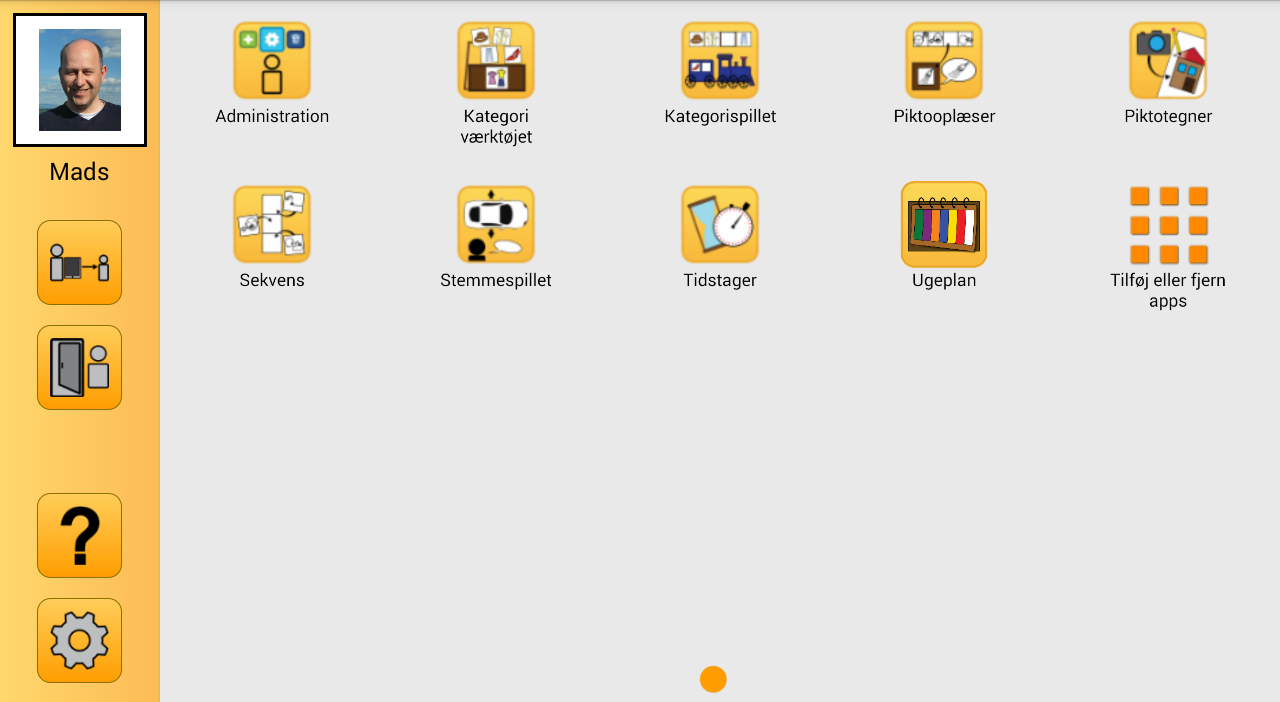
\includegraphics[width=\textwidth]{figures/img/screenshots/addapps_icon.png}
    \caption{Screenshot of the homescreen shown to a guardian. The new pseudo application for managing apps, can be seen in the buttom row on the far right.}\label{fig:addapps}
\end{figure}
